% ----------------------------------------------------------------------
% Section 4 — Hardware
% ----------------------------------------------------------------------
\section{Hardware}\label{sec:hardware}
% TODO: remove section information
% Detailed description of the edge tier of the system.

The sensor node is the physical edge component of the Sensiq system
and is built around an ESP32 microcontroller hosting a set of
environmental sensors that cover temperature, humidity, ambient
light, air pressure, volatile organic compounds (VOCs), flame
radiation and high-temperature events. The following part of this
section first lists the individual hardware components and their
characteristics, then describes the firmware-level measurement
workflow (sensor initialization, periodic sampling, averaging and
MQTT publication), and finally documents the Steinhart--Hart
conversion used for the analog thermistor readings. The resulting
JSON payload sent to AWS IoT Core is described in
\cref{sec:mqtt_publication}.

\subsection*{Component Overview}\label{sec:component_overview}

The following hardware components are used in the sensor node:

\begin{description}
	\item[ESP32 NodeMCU board] Open-source development board carrying
	      the ESP-WROOM-32 module, breaking out 38~pins and providing a
	      CP2102 USB-to-serial bridge for programming and
	      power~\cite{esp32_berrybase}.
	\item[ESP-WROOM-32 module] Xtensa dual-core 32-bit LX6 CPU with up to
	      \SI{240}{\mega\hertz}, \SI{520}{\kilo\byte} SRAM and
	      \SI{4}{\mega\byte} SPI flash; integrated Wi-Fi
	      802.11\,b/g/n with up to \SI{150}{\mega\bit\per\second} and
	      Bluetooth; on-chip 12-bit SAR ADC (analog-to-digital converter) and
	      DAC (digital-to-analog converter). Supplied at
	      \SIrange{3.0}{3.6}{\volt}, operating range
	      \SIrange{-40}{85}{\celsius}~\cite{esp32_wroom_datasheet}.
	\item[DHT11] Single-wire digital temperature/humidity sensor;
	      range \SIrange{-20}{60}{\celsius} at \SI{\pm 2}{\celsius}
	      and \SIrange{5}{98}{\percent}~r.H.\ at
	      \SI{\pm 5}{\percent}~r.H.; sampling at
	      \SI{0.5}{\hertz}~\cite{dht11_asair}.
	\item[Joy-it KY-026 flame sensor] Detects flames in the IR band
	      \SIrange{760}{1100}{\nano\metre} with a \SI{60}{\degree}
	      detection cone up to \SI{100}{\centi\metre}. Provides an
	      inverted analog output (sampled by the ESP32 ADC) and a
	      potentiometer-adjustable digital threshold output for
	      event-driven triggering~\cite{ky026_joyit}.
	\item[Joy-it KY-028 thermistor] NTC temperature sensor covering
	      \SIrange{-55}{125}{\celsius} at \SI{\pm 0.5}{\celsius}.
	      Exposes an analog reading (ADC-limited rate) and a digital
	      over-temperature flag with adjustable
	      threshold~\cite{ky028_joyit}.
	\item[TSL2561 light sensor] Digital I\textsuperscript{2}C
	      ambient-light sensor with two photodiodes (visible and IR);
	      \SIrange{0.1}{40000}{\lux} at \SI{0.1}{\lux}
	      resolution~\cite{tsl2561_datasheet}.
	\item[Bosch BME680] Low-power I\textsuperscript{2}C/SPI sensor combining
	      temperature (\SI{\pm 1.0}{\celsius}), humidity
	      (\SI{\pm 3}{\percent}~r.H.), pressure
	      (\SI{\pm 0.6}{\hecto\pascal}) and a VOC gas channel
	      (\SIrange{2}{5}{\percent} accuracy for ethane, isoprene,
	      ethanol, acetone, CO) exposed as an IAQ index. Configurable
	      update rate up to \SI{1}{\hertz}; operating range
	      \SIrange{-40}{85}{\celsius} and
	      \SIrange{300}{1100}{\hecto\pascal}~\cite{bme680_bosch}.
	\item[Auxiliary switches] Two switches reserved for future work
	      on AI-based outlier detection with gathered training data
	      (see \cref{sec:summary}): one marks a reading as a labeled
	      training sample, the other flags a measurement as an
	      outlier.
\end{description}

The hardware design of the sensor node is presented from three
complementary perspectives.
\Cref{fig:hardware-circuit} shows the logical
circuit diagram made with the KiCAD software~\cite{kicad_software}and documents how the ESP32-DevKitC is wired to the
sensors, the two auxiliary switches and
the power supply, including the GPIO assignment of each signal
line.
\Cref{fig:hardware-pcb} in turn shows the resulting printed circuit board (PCB)
layout with the physical placement of the components, the routed
copper traces and the board outline intended for fabrication.
Both views are exported from the same KiCAD project and together
relate the firmware-level GPIO numbers used in the measurement
workflow to the corresponding physical pads on the planned PCB.
The PCB has not been manufactured yet, so the actual sensor node
shown in \cref{fig:hardware-picture} is built on a prototyping
board with the components manually placed and wired according to
the circuit diagram.

\begin{figure*}[!tb]
	\centering
	
\includegraphics[width=0.8\textwidth]{circuit_diagram_export_light.pdf}
	\caption{Circuit diagram of the sensor node, showing the
		logical wiring between the ESP32-DevKitC, sensors, the two
		auxiliary switches and the power supply, together with their
		respective GPIO assignments.}
	\label{fig:hardware-circuit}
\end{figure*}

\begin{figure}[htb]
	\centering
	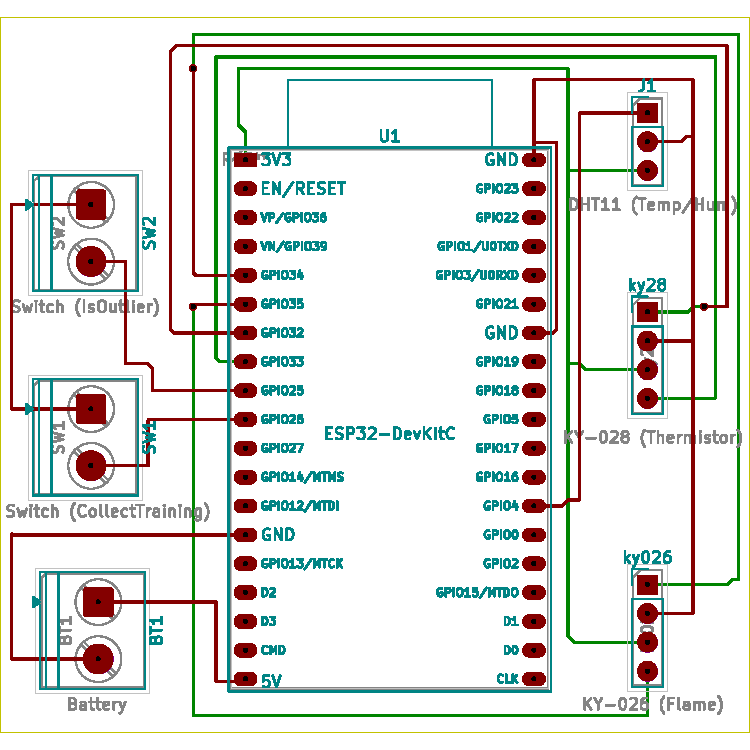
\includegraphics[width=0.95\linewidth]{pcb_pdf_export_light.pdf}
	\caption{PCB layout derived from the circuit diagram, showing
		the physical placement of the ESP32-DevKitC and the
		attached sensors, the routed copper traces and the board
		outline intended for fabrication.}
	\label{fig:hardware-pcb}
\end{figure}

\begin{figure}[htb]
	\centering
	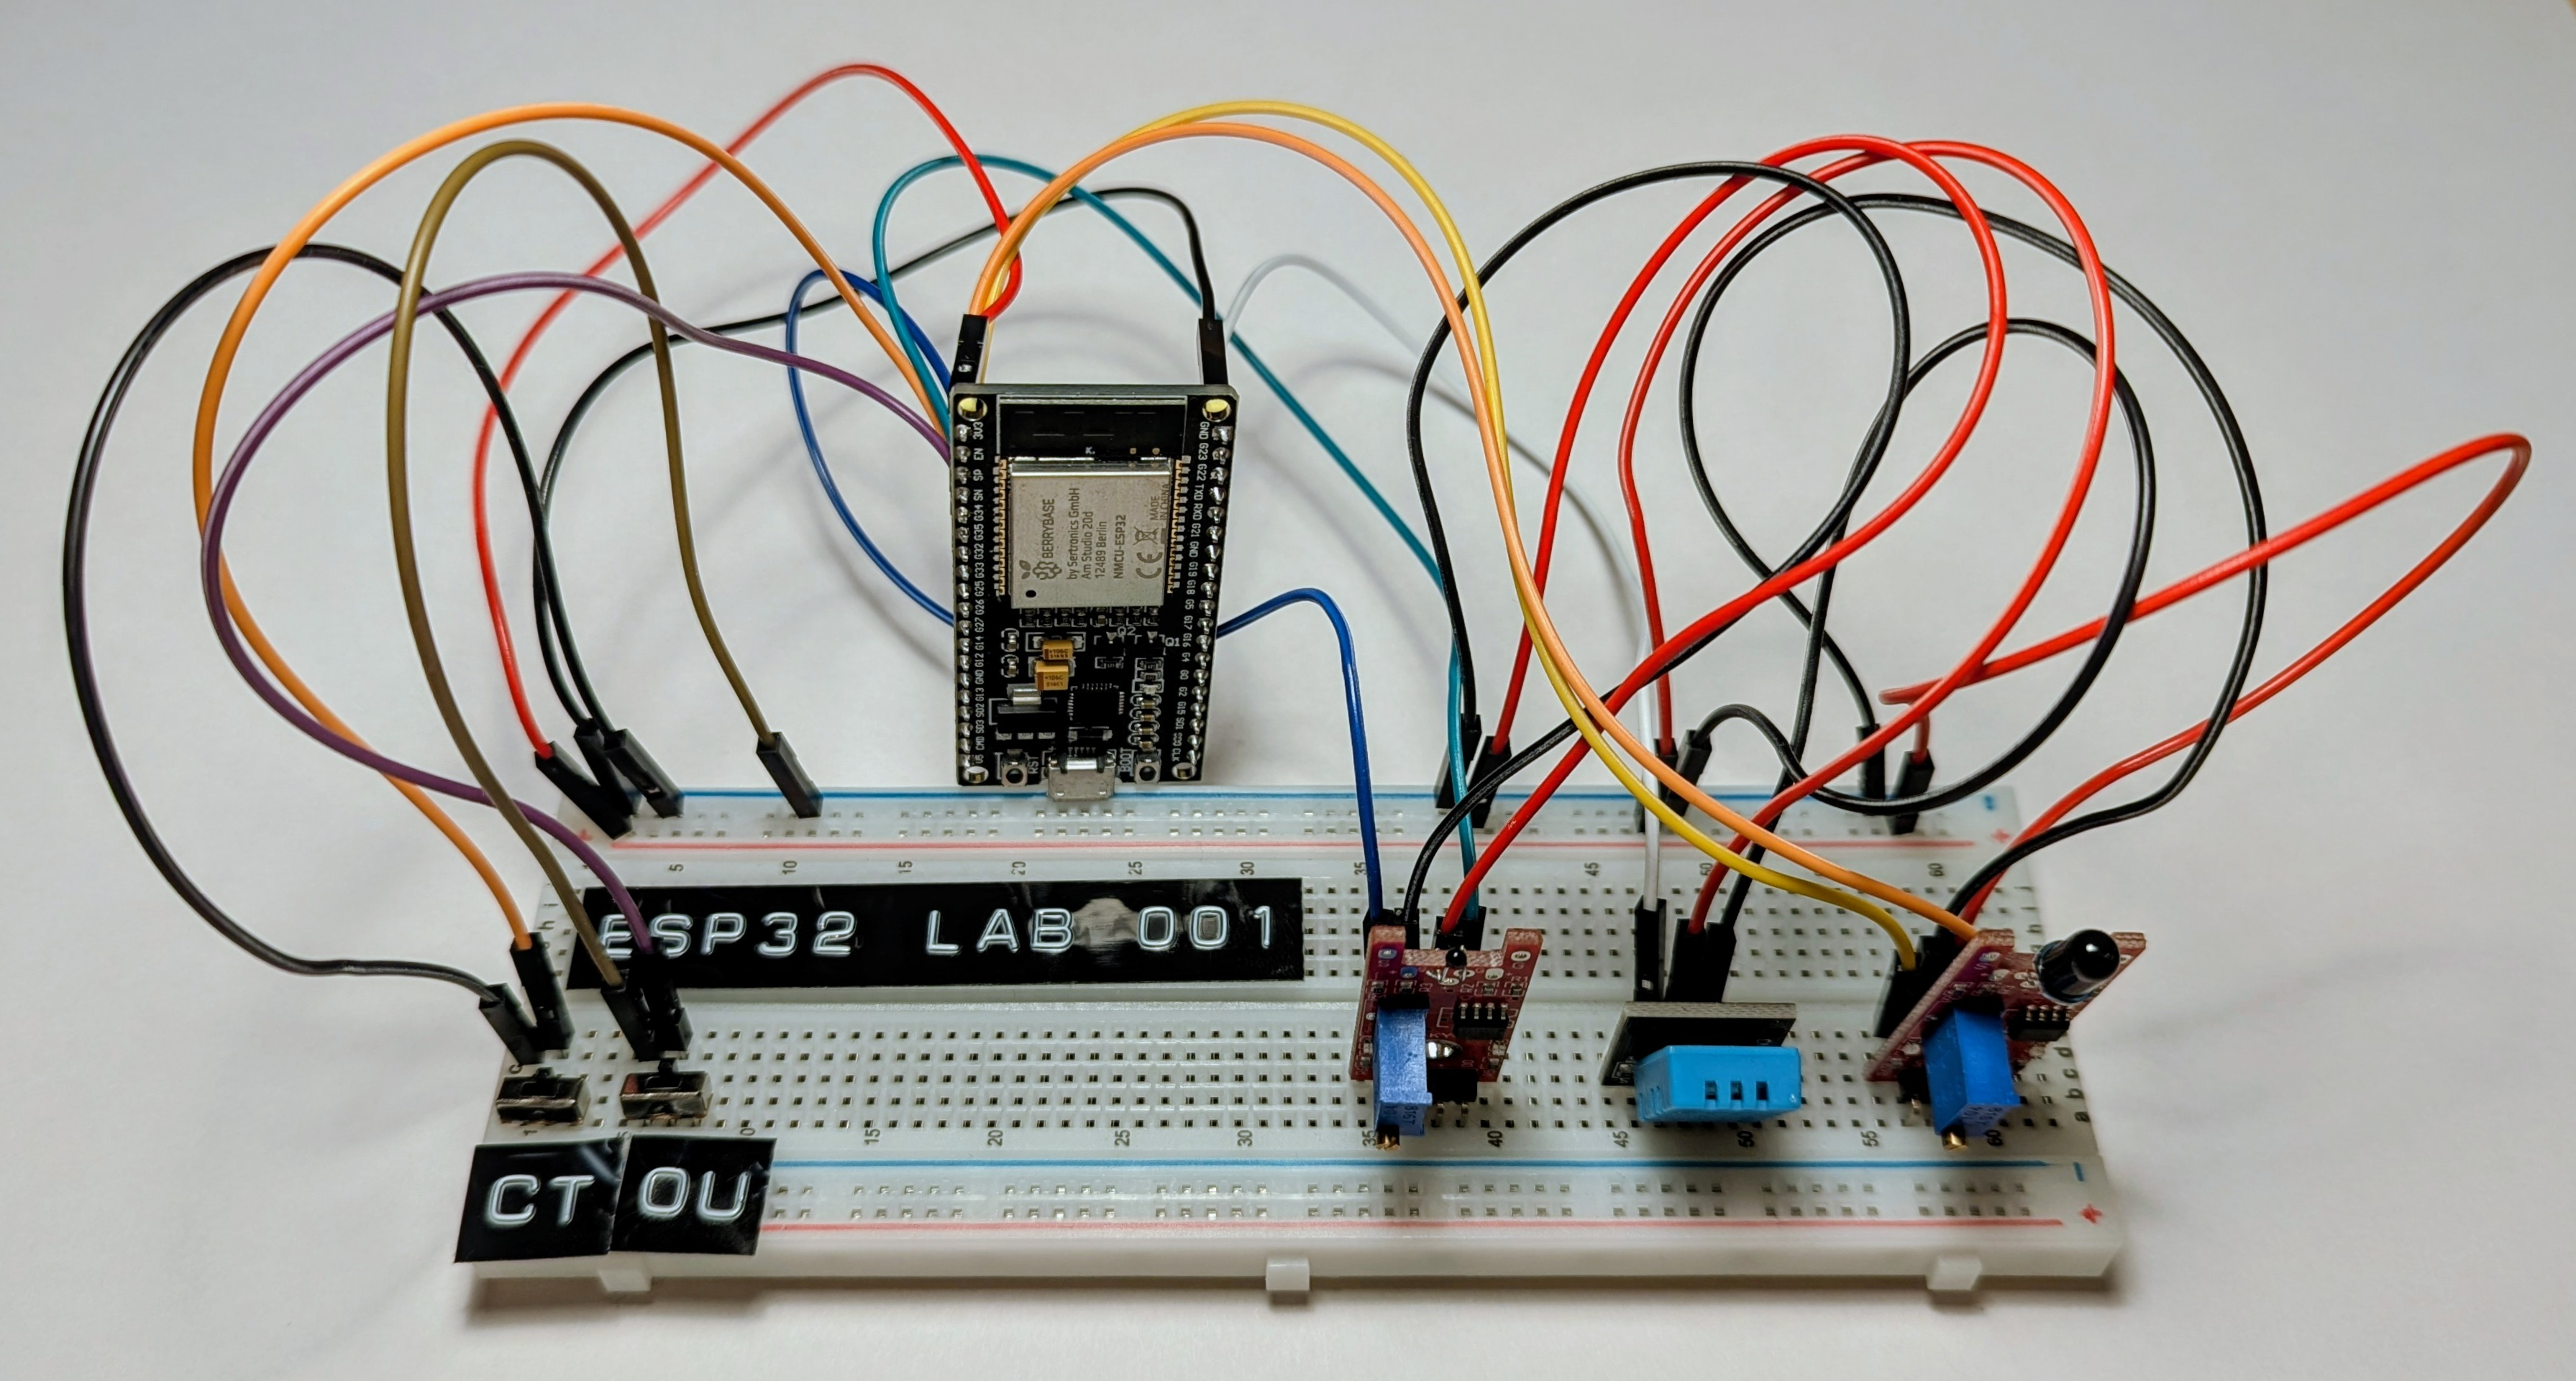
\includegraphics[width=0.95\linewidth]{hardware-picture.png}
	\caption{Real physical sensor node with the assembled sensors,
		the ESP32-DevKitC and the auxiliary switches.}
	\label{fig:hardware-picture}
\end{figure}

\subsection*{Measurement Workflow}\label{sec:measurement_workflow}
The firmware on the ESP32 follows a deterministic, two-phase
lifecycle written in Arduino C++~\cite{arduino_language_reference}:
a one-time \emph{startup} phase that prepares the
networking and sensing subsystems, followed by a continuously running
\emph{measurement loop}.

During startup the node performs the following steps in order:
\begin{enumerate}[leftmargin=*]
	\item Wi-Fi association: The node connects to a
	      configured local network using a pre-provisioned SSID and
	      password.
	\item Time synchronization: The internal clock is
	      synchronized with an NTP server. An accurate wall-clock
	      time is required both for meaningful measurement timestamps
	      and for the validation of TLS certificates during the
	      subsequent MQTT handshake.
	\item Sensor initialization: GPIO pin modes are set and
	      sensor-specific configuration (e.g. DHT11 configuration) is applied.
	\item MQTT setup: The MQTT client is configured (see~\cref{sec:mqtt_publication}).
\end{enumerate}

% small space for better readability
\medskip

Once startup is complete, the node enters its measurement loop:
\begin{itemize}[leftmargin=*]
	\item The MQTT connection is continuously validated and kept
	      alive; on disconnect, the client transparently reconnects.
	\item Every $t$ milliseconds a full sensor reading is taken
	      across all attached sensors with a default waiting period
	      of $t=\SI{1000}{\milli\second}$. Values smaller than one
	      second might not change much, as the sensors often have a
	      minimum sampling rate of \SI{1}{\hertz} or lower.
	\item After $n$ consecutive readings the buffered samples are
	      aggregated into a single record, serialized as JSON and
	      published to the configured MQTT topic. The standard
	      sample aggregation size is $n=5$, guaranteeing a balance
	      between responsiveness and noise reduction.
\end{itemize}
\medskip

Aggregation reduces sensor noise and the influence of isolated
outliers. It is performed per field according to its data type:
the most recent timestamp of the buffer is taken as the record
timestamp, numerical values (analog readings) are averaged
arithmetically, and digital boolean signals are decided by majority
voting over the buffered samples.

\medskip
\subsubsection*{Thermistor Conversion}

The KY-028 module exposes the thermistor as an analog voltage divider
that the ESP32 reads through its 12-bit ADC. The raw ADC value
$\mathrm{adc}\in[0,4095]$ is first converted to a resistance
$R$ assuming a sensor--internal \SI{10}{\kilo\ohm} pull-down resistor and a
\SI{3.3}{\volt} supply, and then to an absolute temperature using the
Steinhart--Hart equation~\cite{steinhart1968calibration}.
The equation models the resistance--temperature relationship of a
semiconductor thermistor as

\begin{equation}
	\frac{1}{T} = A + B \ln R + C (\ln R)^{3},
	\label{eq:steinhart_hart}
\end{equation}

where $T$ is the temperature in kelvin, $R$ is the thermistor
resistance in ohms at temperature $T$, and $A$, $B$ and $C$ are the
Steinhart--Hart coefficients characteristic of the specific
thermistor over the temperature range of interest. The firmware
uses the coefficients $A=1.129148\cdot 10^{-3}$,
$B=2.34125\cdot 10^{-4}$ and $C=8.76741\cdot 10^{-8}$, then converts
$T$ from kelvin to degrees Celsius before further using the value as
\texttt{thermistor\_temp}.

\subsection{MQTT Publication to AWS IoT Core}\label{sec:mqtt_publication}

The sensor node communicates with AWS IoT Core via the MQTT protocol over TLS.
% While an asynchronous MQTT client such as AsyncMQTT\_Generic \cite{asyncmqtt_generic_arduino}
% would theoretically offer non-blocking background execution and better performance
% during unstable connections, it currently lacks support for the required
% AWS IoT Core TLS certificates and is no longer maintained.
% Instead, the firmware utilizes the officially recommended MQTT library by
% Joel Gaehwiler~\cite{arduino_mqtt}, which provides only a synchronous API.

To establish a secure connection to the AWS IoT broker on port 8883,
the node requires the broker address and a set of cryptographic credentials.
The publicly available AWS Root CA certificate alongside the individual
device certificate and device private key are used for mutual TLS authentication.

% TODO: check if this got more values already.
\begin{lstlisting}[
    language=json, 
    float, 
    caption={Published JSON payload by the ESP32 sensor node via MQTT.}, 
    label={lst:data_model_json}]
{
    "running_time": 9881892,
    "timestamp": "2026-05-25T22:56:12Z",
    "device_id": "esp32-lab-001",
    "location": "Lab A, OTH Amberg-Weiden, 92224 Amberg, Germany",
    "dht_humidity": 61,
    "dht_temperature": 23.8,
    "dht_heat_index": 23.82809,
    "flame_analog": 0,
    "flame_digital": false,
    "thermistor_analog": 2005,
    "thermistor_digital": false,
    "thermistor_temp": 24.05634,
    "is_outlier": false,
    "collect_training": false
}
\end{lstlisting}

The MQTT topic structure is designed around a unique device identifier
(e.g., \texttt{esp32-lab-001}).
Data exchange uses three primary topics:
\texttt{sensiq/<identifier>/data} for publishing the aggregated sensor records,
\texttt{sensiq/<identifier>/test} for verifying connectivity, and
\texttt{sensiq/<identifier>/commands} reserved for receiving subsequent control commands.
\Cref{lst:data_model_json} shows an example of the JSON payload that the ESP32
node publishes to the data topic after each aggregation interval.
